\documentclass[a4paper]{report}
\usepackage{graphicx}
%\graphicspath{ { images/} }
\graphicspath{ {/Users/francisdavey/src/physics/blog/images/}}
\usepackage{amsmath}
\usepackage{tikz}

\setlength{\parindent}{0em}
\setlength{\parskip}{1em}

%htlatex twin1.tex "xhtml,html5,mathjax,charset=utf-8" " -cunihtf -utf8"
%https://www.12000.org/my_notes/faq/LATEX/layout/

\begin{document}
\section*{Setting the scene}
\subsection*{The strange behavour of clocks}
Imagine two people are walking in the mountains. They set off from the same base camp. One goes fairly directly to their destination (shown in green) and the other takes a more scenic route (shown in red). While resting at the end, they compare notes and wonder: how high they have climbed above their base camp and how far did they each travel?

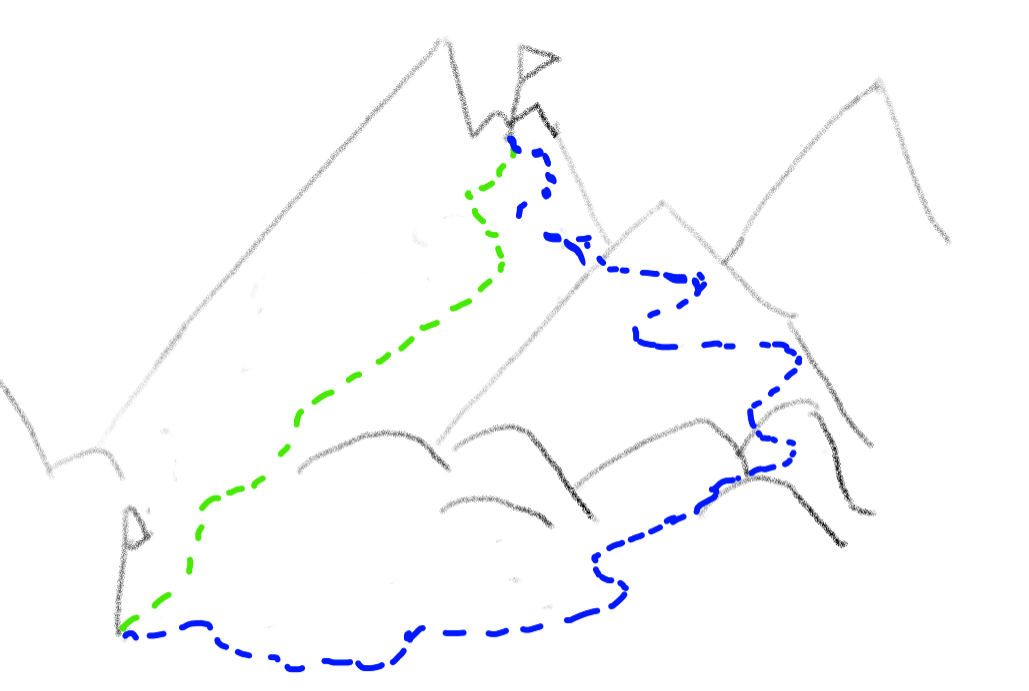
\includegraphics[width=0.5\linewidth]{mountain}

To work out how much higher they are than when they started, all they need to know is wo numbers: the altitude at the start point and at the finish. They can consult a map and substract one from the other to find out how high they have climbed. The answer will be the same for the two travellers because their start and end points are the same. 
How far each has travelled is a different matter. To know that requires knowledge of much more than the start and finish positions, but the whole route. As a child, we would work this sort of thing out by laying pieces of string out on a map as best we could and then straightening them up and measuring them with a ruler. 

We could say altitude climbed is ``path independent'' and distance travelled is ``path dependent''. In mathematical physics, many quantities are either one thing or the other. Realising that something is path independent is often very important, for example  because it makes it easier to compute. 

Another example of something that the climbers will assume is path independent is the duration of their journey. To compute this, so they might think, all they need to know is two things: when they set off; and when they arrived. They can use clocks at the start or destination, or look at their watches (a wearable device for displaying the current time). In particular, if they start and end at the same time, their journies took exactly the same length of time. In other words, the passage of time is path independent.

So at least it was thought for most of human history. Our ancestors were roughly right. For people wandering around in the mountains, catching trains or driving around the countryside, ``time is path independent'' is approximately true. It is not, however, exactly correct. 

%later
Towards the end of the nineteenth century, a number of physicists started to suspect that time was not as straightforward as it looked. The credit for proving that time is path dependent goes to Albert Einstein in 1905. As we shall see later in the series, Einstein could be understood as saying something more like ``time might as well be path dependent for all we know''.

Theory is all very well, but we are now quite sure because of a series of experiments, example Ives-Sitwell. In 1971, four atomic clocks were placed on board commercial airliners and flown around the world. First, twice in the Eastward diretion and then twice in the Westwardy direction. After each trip, the clocks were compared with the time on reference clokcs that did not take the trip. On the Eastward journey, all the clocks ran slow, while going Westward, they all ran fast.

I mention Einstein and the theoreticians because I am telling the story almost backwards. The odd behaviour of clocks -- time dilation as it is sometimes called -- comes nearer the end of the story of relativity. You could start with the theory of electrodynamics and deduce the behaviour of clocks from it. But I think it is easier to see what happens if we start here. 

How does it depend on path? It turns out that all that matters is the velocity along the path - the acceleration and so on does not seem to matter.

To put some numbers in here, if we take, say, a particle in a particle accelerator and see how its velocity affects how quickly it decays, the factor by which it lives long - or if you like its internal clock slows down - is $\sqrt{1 - \frac{v^2}{c^2}}$ where $v$ is the relative velocity and $c$ is the number $299,792,458ms^-1$ or very close to three hundred million metres a second. In order for us to see any of this effect on clocks we need velocities close to this.

$c$ also happens to be the speed of light in a vacuum. In fact that is how it is usually described or defined. But that assumes we know what light is and what it means to say it is travelling in a vacuum. 

To see more about the nature of these numbers, see the extras.

In many popular accounts of relativity for the general public, and I am afraid to say in some more formal situations such as textbooks for university level students, This behaviour of clocks is often expressed roughly as:

\framebox[0.8\linewidth][c]{Moving clocks run slow}

It is, at least, nice and easy: work out how fast a clock is moving and that will tell you how slow it is running. You could say something like: the fast a clock moves in space, the slower it moves in time, or something like that.

However, more sensitive physicists react to this sort of summary with the expression that someone who has just put a lemon in their mouth might have. What is setting their teeth on edge is the rather glib way we are talking about ``moving clocks''. They might say ``moving relative to what''? To really appreciate what they are objecting to, we need to think about an old an important idea known as ``relativity'' and the first person to realy write about it was none other than Galileo Galilii. The second part of our story.

\section*{Galileo's ship}

\includegraphics[width=0.4\linewidth]{genoese_carrack}
% Can we find a painting
%Could we/should we do a diagram

Galileo imagined an experimentalist carrying out their researches in the cabin of a boat. One imagines a large Captain's cabin of the kind seen in romantic descriptions of life in the 18th century navy or as an 18th century pirate. The significant feature is that you cannot see outside. You have no way to know how fast you are travelling. Galileo proposed that no experiment you could carry out inside the cabin would allow you to know the speed with which you were moving.

Another way to put this is that speed is relative. You cannot say ``I am moving at 10m/s'' without saying {\em what} it is that you are moving relative to. If our sailor-physicist's ship were out in the open ocean and they were to step on deck, they could, by dint of various experiments, work out how fast they were moving relative to the ocean, but would not know whether currents in the water were moving the water and thus also the boat floating on it, quickly.

This principle was accepted as a general one in physics and forms a part of Newton's theory (???). (?application to inertial movement only). If relativity were correct, then first of all it would be meaningless to talk about ``moving clocks'', since all movement is relative. But it appears to have a deeper problem. If I move relative to you, you move relative to me. It can't be the case that we both have slower clocks can it?

What more careful explainers of the special theory of relativity say is something more along the liens of 

\framebox{Relatively moving clocks appear to run slow}

The word ``appear'' here is doing a lot of have to do a lot of heavy lifting. It very much does not mean, what it seems to mean. In the next post, I shall unpack what ``appear'' means. But first let us look at the problem of the lack of symmetry between clocks as explained.

\section*{Classic statement of the twin paradox}.

Let us start by imagining two clocks: one goes on journey and returns to its starting point; the other clock stays where it is. As we have explained, there clock that went on a journey goes slower than the clock that stayed behind. This is a fairly startling idea on its own, contradicting as it does many years of philosophy, but a surprise is not a paradox.

The twin paradox plays with the path-dependence of clocks in the context of relativity to create a number of seeming contradictions. Strictly speaking a ``paradox'' is a contradiction - two things that cannot both be true -- whereas here the contradictory points are only seem to be contradictions.

Instead of clocks, let us imagine twins. One stays back at base on Earth - let us call them ``B'' for ``base'' and the other travels to a nearby star system before returning -- let us call them ``A'' for ``astronaut''. Why twins? Well, one of the things we are going to want to do is consider what the world looks like from the point of view of each clock. It is easier to imagine that there are people on the journey able to make observations - clocks not being known for their intelligence.

Twins also seem to be popular because the human body, in aging, is a natural clock. An effect that works on people somehow, I imagine, personalises it.

If A sets off at a speed of 80\% the speed of light relative to the Earth and travels out for 5 years according to the clock back at base, turning around and returning to Earth at the same relative speed, A's clock will be found to be 60\% as fast as B's. A will have aged 6 years, while B has aged 10. The relationship is $\sqrt(1 - \frac{v^2}{c^2})$ where $v$ is the velocity and $c$ is the speed of light. We picked 80\% of course because the numbers came out nicely.

Now it seems to me that there are actually three different things about this story that cause people to scratch their heads - some of them immediately and others after thinking about it for a while. All, or any of these, could be the ``paradox''.

First, we might say that this story is all about A moving relative to B at 80\% the speed of light. But surely, if relativity is correct, B is moving relative to A at 80\% of the speed of light throughout. Surely then B's clock ought to be slower than A's, which is a contradiction.

This is typically met with two responses: first to say that time is not exact. You can't just think about where you start and where you end, but the journey you took. A's journey is different from B's and so their clock is different. You might as well object that two people walking in the mountains as we imagined at the start of this post and who covered different differences on the ground would be entitled to object that each could imagine the other one was moving further.

Another answer is to say that relativity applies only between observers (XX make an earlier note of observer) who do not accelerate. A must have accelerated when they turned around. So that ends the argument. ...

These arguments can risk sounding as if they are saying ``well, it is just like that''. Many students want to see exactly what happens - don't worry, we will will look very carefully at that, which in turn leads to another question.

While A is travelling away - and yet again when they are returning - A is an inertial (XX metion this) observer. They are entitled, under the rules we have explained above, to say that B's clock runs slower than theirs. If moving clocks appear to run slow, then A can see B's clock appearing to run slow for most of the journey, yet at the end of the journey A can see their clock actually recorded less time.

Where did the time go? Does it realy just vanish (or appear) at the moment of turn around as the ``it is all about acceleration'' explanation has it.  And how can that seeming asymmetry work? Surely at some point A must think B's clock is running fast or something is very wrong.

So we have three things to explain: why exactly can't A turn the story around and talk about it from their point of view? How can both A and B think the other's clock is slow and where did the time go? What is very rarely explained in courses on special relativity is that none of these three seemingly paradoxical questions have all that much to do with special relativity. The asymmetry between A and B, and indeed something very like the twin paradox, can be described in an entirely Newtonian universe. Doing so has one big advantage: you do not need to worry about there being some mysterious relativistic effects going on that you don't yet understand. It can't (for example) be because accelerating objects must be dealt with using general relativity (a popular idea at one stage).

\section*{The Galilean Twin Paradox}

So, we will attack this paradox in stages. First, let us imagine a world where Newton's laws apply and Galilean relativity is the only relativity available. We make two assumptions about the physical behaviour of light (by which we mean all electromagnetic energy, including radio waves):
\begin{itemize}
\item The speed with which light travels does not depend on how fast the source of the light is moving.
\item The speed of light does not depend on the direction.
\end{itemize}

Both these assumptions agree with experiment (which ones?) and the theory of electromagnetism. We are not assuming that the speed of light is identical for every observer.



% Slow clock outward journey
So, what does each astronaut see at the start of B's journey? Rather than trying to imagine each continuously viewing each other's clock with a telescope or other means of distance viewing, let each astronaut send out a ``tick'' every second from their clock in the form of a radio (light) pulse.

Regardless of the state of her clock, B will see A's light pulses arriving more slowly than they were transmitted because each pulse takes slightly longer to reach her as she moves away from A.

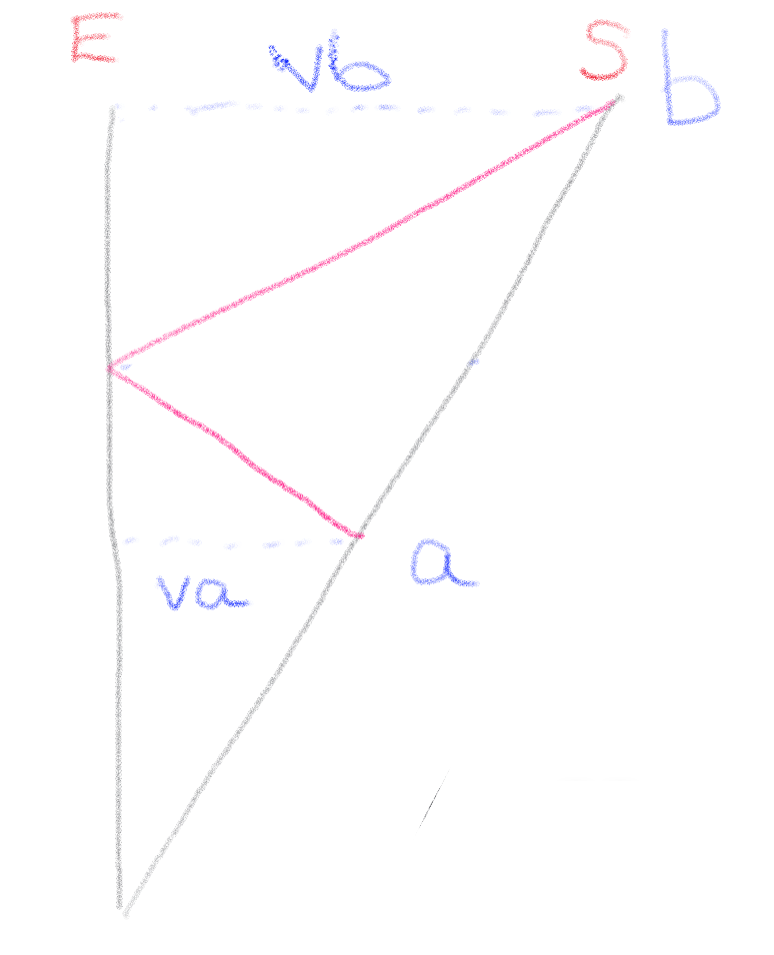
\includegraphics[width=5cm]{sketch2}

% Use radar (or sonar) Relative velocity (as a fraction of c) does not depend on clock
% What B "sees", what A "sees". Doppler effect.
% Applying Doppler effect, now what happens if we assume slow clock?

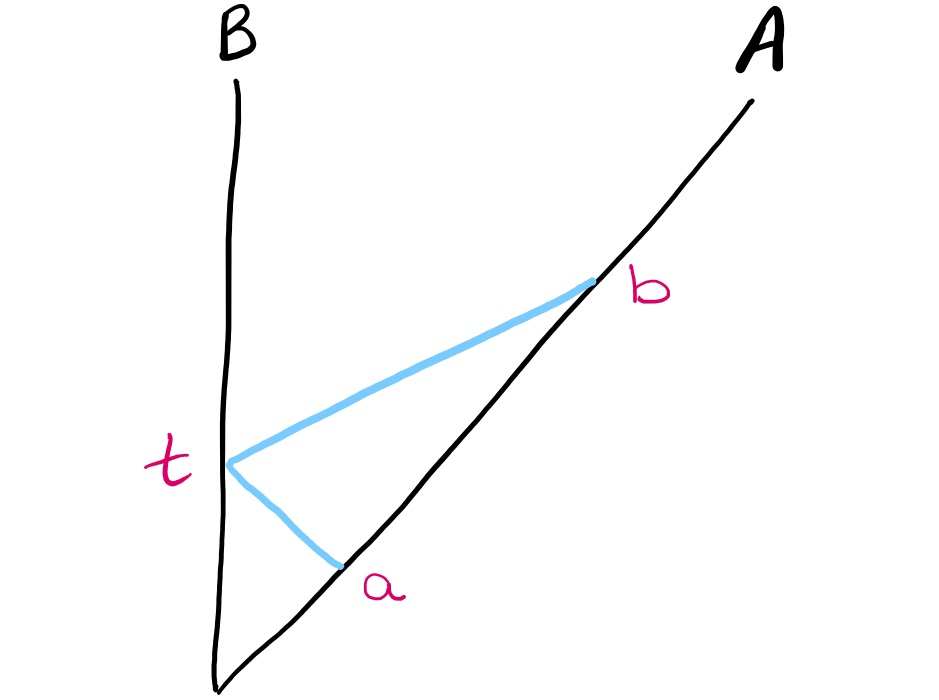
\includegraphics[width=5cm]{relative_velocity_b}
\begin{align*}
  (t - a) c & =  av \\
  t & = a(1 + \beta) \\
(b - t)c & =  bv \\
t & = b(1 - \beta) \\
a(1 + \beta) & = b(1 - \beta) \\
\beta(a + b) & = b - a \\
\beta & = \frac{b - a}{b + a} 
\end{align*}

Thus the relative velocity as a fraction of $c$ can be computed without reference to whether or not A's clock is slow.

% Symmetry, even though we know that there is an asymmetry. This is at the root of the twin paradox. There is a fundamental symmetry

Applying the Doppler effect.

\begin{tikzpicture}
  \coordinate (A) at (0,0);
  \draw (A) -- +(0, 3) node[pos=1,above] {B};
  \draw (A) -- (2, 3) node[pos=0.666] (sa) {} node[pos=1,above] {A};
  \draw (-0.5, 1) node[left] {$t_B$} -- (0.5, 1);
  \draw (sa) -- +(-0.5, 0) -- +(0.5, 0) node[right] {$s_B$};
  %\draw (sa) -- +(0.5, 0);
\coordinate (RO) at (8,0);
  \draw (RO) -- +(0, 3) node[pos=1,above] {A};
  \draw (RO) -- +(-2, 3) node[pos=0.666] (tb) {} node[pos=1,above] {B};
  \draw (7.5, 1)  -- (8.5, 1) node[pos=1, right] {$s_A$};
  \draw (tb) -- +(-0.5, 0) -- +(0.5, 0) node[pos=0, left] {$t_A$};
\end{tikzpicture}

\begin{equation*}
  \begin{aligned}[c]
    \begin{tikzpicture}
      \coordinate (A) at (0,0);
      \draw (A) -- +(0, 3) node[pos=1,above] {B};
      \draw (A) -- (2, 3) node[pos=0.666] (sa) {} node[pos=1,above] {A};
      \draw (-0.5, 1) node[left] {$t_B$} -- (0.5, 1);
      \draw (sa) -- +(-0.5, 0) -- +(0.5, 0) node[right] {$s_B$};
    \end{tikzpicture}\\
%\intertext{B's picture from the base}
    s_Bv &=(s_B - t_B)c \\
s_B (1 - \beta) &=t_B \\
s_B & = \frac{t_B}{1 - \beta} 
  \end{aligned}
  \begin{aligned}[c]
    \begin{tikzpicture}
      \coordinate (RO) at (8,0);
      \draw (RO) -- +(0, 3) node[pos=1,above] {A};
      \draw (RO) -- +(-2, 3) node[pos=0.666] (tb) {} node[pos=1,above] {B};
      \draw (7.5, 1)  -- (8.5, 1) node[pos=1, right] {$s_B'$};
      \draw (tb) -- +(-0.5, 0) -- +(0.5, 0) node[pos=0, left] {$t_B'$};
    \end{tikzpicture} \\
    t_B' v&= (s_B'-t_B')c \\
    t_B'(v + c) &= s_B'c \\
t_B'&=\frac{s_B'}{a+\beta} 
  \end{aligned}
%t_B'&=&\frac{k}{1-\beta^2}
\end{equation*}
Combining the two gives us:
\begin{align*}
  t_B'&=\frac{kS_B}{1 + \beta} \\
&=\frac{kt_B}{1-\beta^2}
\end{align*}

If $k > 1 - \beta^2$ then B's clock will appear to run slow for A, even though A's clock is in fact running slow. If $k = \sqrt{1 - \beta^2}$ then A and B will each see the other's clock running slow at exactly the same rate.

Here we see that even in the Newtonian world, provided the moving clock runs slow at exactly the right rate, we have the asymmetry of the Twin Paradox.

Having a slow clock will mean mistiming the speed of light.

% Would like to jump in right now and apply to twin paradox.
% Whole setup.
% Twin paradox a bit more difficult because we don't know relative velocity for most of the trip. Use of radar does not work.

A can use this system of radar to work out both the time and distance of an event (define event), by sending a radar beam to it and then receiving one back. This will give the Lorentz Transformation.

(demonstrate Lorentz transformation or leave until extras)

In the twin paradox, A does not know the relative velocity so easily throughout the journey because for a part of the journey, radar sent from A on its outer journey, will be received by it on its return journey. Similarly it cannot use a system of radar to find the location of distant objects and so cannot reason about B.

If A uses radar nonetheless, it discovers:

(relative velocity)

(space-time diagram)

An alternative approach is to  Clock paradox (three clocks paradox). Radar stations. Convenient. Overlap problem (but we don't mind for now). Can now work out relative velocity and dedice timing of other clock by application.

% Out - short. In - long. ??? HOw does this resolve PROBLEM.


\section*{Moving clocks run slow world}
% Lorentz transformation
% Not relativity
Could observe using other laws of physics.
% Rods not clocks
\section*{extras}

% Hafele experiment
% http://www.personal.psu.edu/rq9/HOW/Atomic_Clocks_Predictions.pdf

\subsection*{Using Sonar}
To really make the point that the conceptual problems of the twin paradox can appear in the Galilean/Newtonian world, I had considered telling the story of the twins using sonar rather than radar.

In this version, A is an aviator who leaves behind her twin B who stays back at base. A is now only able to use sonar to determine the distance and relative speed of B. In order for this to work we would have to assume that the speed of sound was uniform and isotropic, for example by assuming that air pressure, temperature and so on were uniform throughout the experiment.

The problem is that this is a harder thought experiment to imagine. While the emptiness of space is strictly speaking not empty at all even in the classical world, let alone when one considers the quantum vacuum, it is easier to imagine than for an aeroplane. It is also the case that either there is no ether to detect or if it exists we cannot direclty observe it, yet it is fairly easy for an aeroplane to detect their air speed (moving air being something we are deliberately not thinking about).

But sound waves also travel with a speed which is source independent and given the right conditions have isotroptic and uniform velocity (query: what does isotropic mean precisely). An aviator using sonar in the same way as radar and who has a slow clock will see all the same behavoiur as their faster moving counterpart up to and including the Lorentz transformation. 

Sound does not quite work this way becuase the pressure of the air, its humidity etc cause the speed of sound to vary. So let us imagine an entirely featureless, flat, world with uniform air pressure, so that sound obeys these principles too. We will call the speed of sound or light in these circumstances $c$ (it's just a number).

Note: reference to air and ether here, perhaps go back and say something about this with the water earlier?


\end{document}
